% ===================================================================
%  Week 16 — Session 1: Transfer Learning
%  Compile: pdflatex -interaction=nonstopmode slides-a.tex  (twice)
% ===================================================================
\documentclass[10pt,aspectratio=169]{beamer}
% ===================================================================
%  Shared Beamer preamble for "Practical Image Processing"
%  English slides. Compile with pdfLaTeX.
% ===================================================================

\usetheme{metropolis}
\usepackage[T1]{fontenc}
\usepackage[utf8]{inputenc}
\usepackage{lmodern}
\usepackage{listings}
\usepackage{tcolorbox}
\usepackage{fontawesome5}
\usepackage{booktabs}
\usepackage{amsmath,amssymb}
\usepackage{tikz}
\usepackage{pgfplots}
\pgfplotsset{compat=1.17}
\usetikzlibrary{arrows.meta,positioning,shapes.geometric,fit,backgrounds,matrix}
\tcbuselibrary{skins,breakable}

% ---- Palette --------------------------------------------------------
\definecolor{coursePrimary}{HTML}{1B4965}   % deep blue
\definecolor{courseAccent}{HTML}{E76F51}    % coral
\definecolor{courseGood}{HTML}{2A9D8F}      % teal
\definecolor{courseBad}{HTML}{C0392B}       % red
\definecolor{courseInfo}{HTML}{2980B9}      % blue
\definecolor{codeBg}{HTML}{F5F6FA}
\definecolor{codeKw}{HTML}{8E44AD}
\definecolor{codeStr}{HTML}{2A9D8F}
\definecolor{codeCom}{HTML}{7F8C8D}

\setbeamercolor{frametitle}{bg=coursePrimary}
\setbeamercolor{progress bar}{fg=courseAccent}
\setbeamercolor{alerted text}{fg=courseAccent}
\metroset{block=fill,sectionpage=progressbar,numbering=fraction}

% ---- Code listings (Python is built into listings) -----------------
\lstdefinestyle{course}{
  backgroundcolor=\color{codeBg},
  basicstyle=\ttfamily\scriptsize,
  keywordstyle=\color{codeKw}\bfseries,
  stringstyle=\color{codeStr},
  commentstyle=\color{codeCom}\itshape,
  numberstyle=\tiny\color{codeCom},
  numbers=left, numbersep=6pt,
  showstringspaces=false, breaklines=true, breakatwhitespace=true,
  tabsize=4, columns=fullflexible,
  frame=single, framesep=4pt, rulecolor=\color{gray!30},
  keepspaces=true, upquote=true, language=Python,
}
\lstset{style=course}
\lstdefinelanguage{bash}{
  keywords={cd,pip,python,venv,source,import}, sensitive=true,
  morecomment=[l]{\#}, morestring=[b]', morestring=[b]",
}

% ---- Reusable callout boxes ----------------------------------------
\newtcolorbox{goodbox}[1][Good practice]{colback=courseGood!8,colframe=courseGood,
  fonttitle=\bfseries,title={\faCheck~#1},boxrule=0.6pt,left=4pt,right=4pt,top=3pt,bottom=3pt}
\newtcolorbox{badbox}[1][Pitfall]{colback=courseBad!8,colframe=courseBad,
  fonttitle=\bfseries,title={\faTimes~#1},boxrule=0.6pt,left=4pt,right=4pt,top=3pt,bottom=3pt}
\newtcolorbox{infobox}[1][Note]{colback=courseInfo!8,colframe=courseInfo,
  fonttitle=\bfseries,title={\faInfoCircle~#1},boxrule=0.6pt,left=4pt,right=4pt,top=3pt,bottom=3pt}
\newtcolorbox{mathbox}[1][Math]{colback=coursePrimary!6,colframe=coursePrimary,
  fonttitle=\bfseries,title={\faCalculator~#1},boxrule=0.6pt,left=4pt,right=4pt,top=3pt,bottom=3pt}

\newcommand{\keyidea}[1]{\begin{alertblock}{Key idea}#1\end{alertblock}}
\newcommand{\term}[1]{\textbf{\color{coursePrimary}#1}}
\newcommand{\code}[1]{\lstinline[basicstyle=\ttfamily\small]|#1|}

% ---- A helper to draw a small pixel grid, cells shaded by value ----
% \pixelgrid{ {10,20,120,200,240}, {30,60,130,180,230}, ... }
\newcommand{\pixelgrid}[1]{%
  \begin{tikzpicture}[font=\scriptsize,scale=0.6]
    \foreach \row [count=\ry] in {#1} {
      \foreach \val [count=\cx] in \row {
        \draw[gray,fill=coursePrimary!8] (\cx,-\ry) rectangle ++(1,-1);
        \node at (\cx+0.5,-\ry-0.5) {\val};
      }
    }
  \end{tikzpicture}}


\title{Transfer Learning \& the DocScan Capstone}
\subtitle{Week 16 — Session 1: Standing on a giant's shoulders}
\author{Practical Image Processing}
\date{Lecture 16.1 \textbullet\ 60--70 min}

\begin{document}

\maketitle

\begin{frame}{Where we stand}
  \begin{columns}[T]
    \begin{column}{0.58\textwidth}
      \begin{itemize}
        \item Week 12: HOG+SVM plateaued at \textbf{0.48} on look-alike cars.
        \item Week 13: CNNs learn features end-to-end — but need lots of data.
        \item \alert{Today:} \term{transfer learning} — reuse a net trained on millions of
              images so a tiny dataset still gets deep-learning power.
      \end{itemize}
    \end{column}
    \begin{column}{0.42\textwidth}
      \begin{alertblock}{Today's real result}
        Same cars, same SVM, but \term{deep features} from a pretrained net:
        \textbf{0.48 $\rightarrow$ 0.87}.
      \end{alertblock}
    \end{column}
  \end{columns}
\end{frame}

\begin{frame}{Roadmap}\tableofcontents\end{frame}

% ==================================================================
\section{The small-data problem}
% ==================================================================

\begin{frame}{Why we can't just train a big CNN}
  \begin{itemize}
    \item Deep CNNs have millions of parameters and want $10^4$--$10^6$ labelled images.
    \item We have \textbf{60 images per car model} — training a big net from scratch would
          memorize, not generalize.
    \item Yet the HOG ceiling (0.48) proves hand features aren't enough. What now?
  \end{itemize}
  \keyidea{Most real projects have \emph{small} data. Transfer learning is how you still use deep learning.}
\end{frame}

\begin{frame}{Parameters vs.\ examples: a feel for the gap}
  \begin{columns}[T]
    \begin{column}{0.54\textwidth}
      \begin{mathbox}[Rough rule]
        You want at least a handful of examples \emph{per free parameter}. A net with
        $P$ parameters and $N$ examples is in danger when $N \ll P$.
      \end{mathbox}
      \begin{itemize}
        \item ConvNeXt-Tiny: $P \approx 28{,}000{,}000$.
        \item Our data: $N = 180$ images total.
        \item $N/P \approx 6\times10^{-6}$ — hopeless from scratch.
      \end{itemize}
    \end{column}
    \begin{column}{0.46\textwidth}
      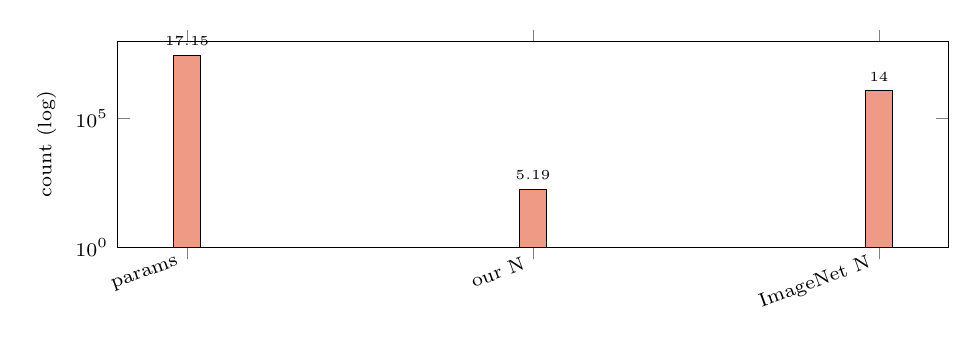
\begin{tikzpicture}[font=\scriptsize]
        \begin{axis}[width=\linewidth,height=4.2cm,
            ybar,ymode=log,ymin=1,ymax=1e8,
            symbolic x coords={params,our N,ImageNet N},
            xtick=data,x tick label style={rotate=20,anchor=east},
            ylabel={count (log)},nodes near coords,every node near coord/.append style={font=\tiny}]
          \addplot[fill=courseAccent!70] coordinates
            {(params,28000000) (our N,180) (ImageNet N,1200000)};
        \end{axis}
      \end{tikzpicture}
    \end{column}
  \end{columns}
\end{frame}

\begin{frame}{What overfitting looks like}
  \begin{columns}[T]
    \begin{column}{0.5\textwidth}
      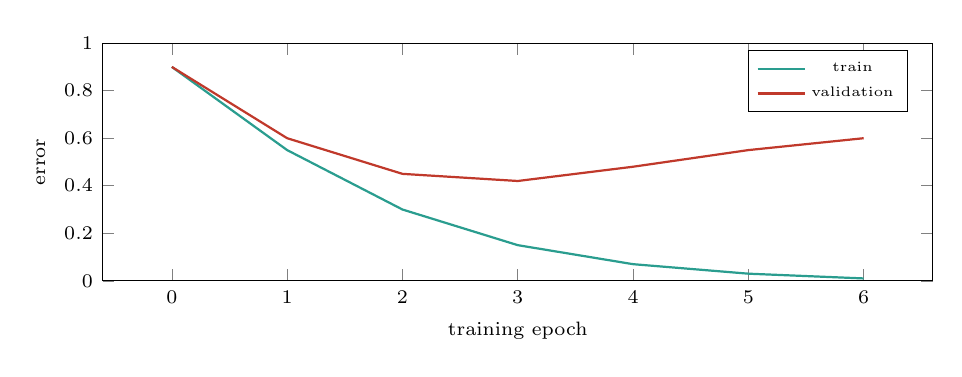
\begin{tikzpicture}[font=\scriptsize]
        \begin{axis}[width=\linewidth,height=4.6cm,
            xlabel={training epoch},ylabel={error},
            ymin=0,ymax=1,legend pos=north east,legend style={font=\tiny}]
          \addplot[courseGood,thick] coordinates
            {(0,0.9)(1,0.55)(2,0.3)(3,0.15)(4,0.07)(5,0.03)(6,0.01)};
          \addlegendentry{train}
          \addplot[courseBad,thick] coordinates
            {(0,0.9)(1,0.6)(2,0.45)(3,0.42)(4,0.48)(5,0.55)(6,0.6)};
          \addlegendentry{validation}
        \end{axis}
      \end{tikzpicture}
    \end{column}
    \begin{column}{0.5\textwidth}
      \begin{itemize}
        \item Training error keeps dropping toward zero.
        \item Validation error bottoms out, then \emph{rises} — the net memorizes noise.
        \item With 180 images this happens in a few epochs.
      \end{itemize}
      \begin{badbox}
        A tiny gap on train tells you nothing. Always watch the \emph{validation} curve.
      \end{badbox}
    \end{column}
  \end{columns}
\end{frame}

% ==================================================================
\section{The key insight: reuse features}
% ==================================================================

\begin{frame}{The key insight}
  \begin{itemize}
    \item A CNN trained on ImageNet (1.2M images, 1000 classes) learned \emph{general}
          visual features: edges, textures, shapes, parts.
    \item Those early/mid features are useful for \emph{almost any} image task — cars included.
    \item So: \term{reuse} those learned features instead of learning them from scratch.
  \end{itemize}
  \keyidea{The first layers of a good vision net are a general-purpose feature extractor. Don't waste them.}
\end{frame}

\begin{frame}{Anatomy of reuse}
  \begin{center}
  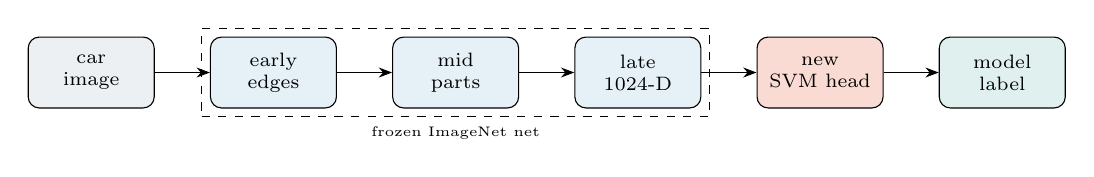
\begin{tikzpicture}[font=\scriptsize,>=Stealth,node distance=4mm and 7mm,
    b/.style={draw,rounded corners,minimum height=9mm,minimum width=16mm,align=center},
    frozen/.style={b,fill=courseInfo!12},
    warm/.style={b,fill=courseAccent!25}]
    \node[b,fill=coursePrimary!8] (img) {car\\image};
    \node[frozen,right=of img] (e) {early\\edges};
    \node[frozen,right=of e] (m) {mid\\parts};
    \node[frozen,right=of m] (l) {late\\1024-D};
    \node[warm,right=of l] (h) {new\\SVM head};
    \node[b,fill=courseGood!15,right=of h] (y) {model\\label};
    \draw[->](img)--(e);\draw[->](e)--(m);\draw[->](m)--(l);\draw[->](l)--(h);\draw[->](h)--(y);
    \begin{scope}[on background layer]
      \node[draw,dashed,fit=(e)(m)(l),inner sep=3pt,label=below:{\tiny frozen ImageNet net}]{};
    \end{scope}
  \end{tikzpicture}
  \end{center}
  \begin{itemize}
    \item The frozen net is a \emph{fixed function} $\phi:\ \text{image}\to\mathbb{R}^{1024}$.
    \item We only train the small orange head on top — seconds, not hours.
  \end{itemize}
\end{frame}

\begin{frame}{Features are learned, not designed}
  \begin{columns}[T]
    \begin{column}{0.5\textwidth}
      \begin{itemize}
        \item Week 12 HOG: \emph{we} decided to count edge orientations in cells.
        \item A trained net \emph{discovered} its own detectors from data — and better ones.
        \item Visualizing them shows a clear hierarchy from edges to object parts.
      \end{itemize}
    \end{column}
    \begin{column}{0.5\textwidth}
      \begin{center}
      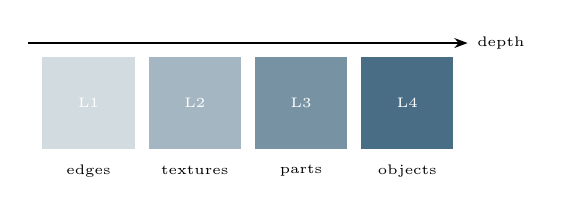
\begin{tikzpicture}[font=\tiny,scale=0.9]
        \foreach \x/\lab in {0/edges,1/textures,2/parts,3/objects}{
          \fill[coursePrimary!\the\numexpr20+\x*20\relax] (\x*1.5,0) rectangle ++(1.3,1.3);
          \node at (\x*1.5+0.65,-0.3){\lab};
          \node[white] at (\x*1.5+0.65,0.65){L\the\numexpr\x+1\relax};
        }
        \draw[->,>=Stealth](-0.2,1.5)--(6.0,1.5) node[right,black]{depth};
      \end{tikzpicture}
      \end{center}
      \begin{infobox}[Same as W6]
        Early filters look like the Gabor/edge kernels we built by hand in the filtering weeks.
      \end{infobox}
    \end{column}
  \end{columns}
\end{frame}

% ==================================================================
\section{Two flavours of transfer learning}
% ==================================================================

\begin{frame}{Feature extraction vs.\ fine-tuning}
  \begin{center}
  \begin{tabular}{@{}lll@{}}
    \toprule
    \textbf{Approach} & \textbf{What you do} & \textbf{When} \\
    \midrule
    Feature extraction & freeze the net, train a new classifier head & very small data \\
    Fine-tuning & unfreeze some top layers, train them too & more data \\
    \bottomrule
  \end{tabular}
  \end{center}
  \begin{itemize}
    \item Today we use \term{feature extraction}: a frozen ImageNet ConvNeXt turns each
          car into a 1024-D vector, then an SVM classifies.
    \item Exactly Week 12's classifier — better features, nothing else changed.
  \end{itemize}
\end{frame}

\begin{frame}{A decision rule you can carry}
  \begin{columns}[T]
    \begin{column}{0.52\textwidth}
      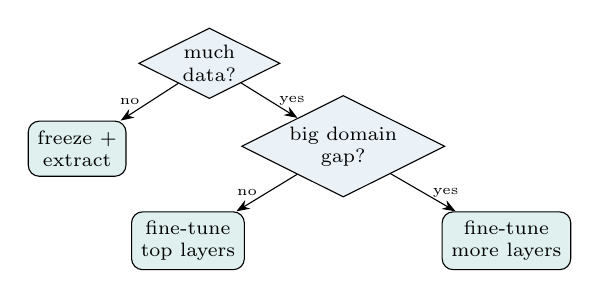
\begin{tikzpicture}[font=\scriptsize,>=Stealth,node distance=5mm and 6mm,
        d/.style={draw,diamond,aspect=2,fill=courseInfo!10,align=center,inner sep=1pt},
        a/.style={draw,rounded corners,fill=courseGood!15,align=center,minimum height=7mm}]
        \node[d](data){much\\data?};
        \node[a,below left=of data](fe){freeze +\\extract};
        \node[d,below right=of data](gap){big domain\\gap?};
        \node[a,below left=of gap](ft1){fine-tune\\top layers};
        \node[a,below right=of gap](ft2){fine-tune\\more layers};
        \draw[->](data)-- node[left,font=\tiny]{no}(fe);
        \draw[->](data)-- node[right,font=\tiny]{yes}(gap);
        \draw[->](gap)-- node[left,font=\tiny]{no}(ft1);
        \draw[->](gap)-- node[right,font=\tiny]{yes}(ft2);
      \end{tikzpicture}
    \end{column}
    \begin{column}{0.48\textwidth}
      \begin{itemize}
        \item Small data $\rightarrow$ never touch the backbone; you would just overfit it.
        \item More data + similar domain $\rightarrow$ fine-tune a few top layers.
        \item More data + distant domain $\rightarrow$ fine-tune deeper.
      \end{itemize}
      \begin{goodbox}
        When unsure, start frozen. It is faster, safer, and a strong baseline.
      \end{goodbox}
    \end{column}
  \end{columns}
\end{frame}

% ==================================================================
\section{The feature-extraction pipeline}
% ==================================================================

\begin{frame}[fragile]{Extracting deep features (code)}
\begin{lstlisting}
import torch, timm
from torchvision import transforms as T

# 1. load a pretrained backbone, drop its classifier
net = timm.create_model("convnext_tiny", pretrained=True,
                        num_classes=0)      # num_classes=0 -> feature vector
net.eval()                                   # freeze: no training

# 2. use the model's OWN preprocessing (must match!)
prep = T.Compose([T.Resize(236), T.CenterCrop(224),
                  T.ToTensor(),
                  T.Normalize(mean=[0.485,0.456,0.406],
                              std =[0.229,0.224,0.225])])

@torch.no_grad()
def features(img):                           # img: PIL RGB
    x = prep(img).unsqueeze(0)               # 1x3x224x224
    return net(x).squeeze(0).numpy()         # -> 1024-D vector
\end{lstlisting}
\end{frame}

\begin{frame}[fragile]{From vectors to a classifier (code)}
\begin{lstlisting}
import numpy as np
from sklearn.svm import SVC
from sklearn.pipeline import make_pipeline
from sklearn.preprocessing import StandardScaler

X = np.stack([features(im) for im in train_images])  # (180,1024)
y = np.array(train_labels)

clf = make_pipeline(StandardScaler(),
                    SVC(C=10, kernel="rbf"))          # same SVM as Week 12
clf.fit(X, y)

Xt = np.stack([features(im) for im in test_images])
print("accuracy:", clf.score(Xt, test_labels))        # ~0.87
\end{lstlisting}
  \begin{itemize}
    \item The \emph{only} change from Week 12 is where \code{X} comes from.
  \end{itemize}
\end{frame}

\begin{frame}{Why standardize the features?}
  \begin{columns}[T]
    \begin{column}{0.55\textwidth}
      \begin{mathbox}[Per-dimension scaling]
        For each feature dimension $j$:
        \[ \tilde{x}_j = \frac{x_j - \mu_j}{\sigma_j} \]
        with $\mu_j,\sigma_j$ estimated on the \emph{training} set only.
      \end{mathbox}
    \end{column}
    \begin{column}{0.45\textwidth}
      \begin{itemize}
        \item Deep features have wildly different scales per dimension.
        \item An RBF-SVM measures distance; unscaled dims dominate it.
        \item Fit the scaler on train, apply to test — never peek at test stats.
      \end{itemize}
    \end{column}
  \end{columns}
  \begin{badbox}
    Fitting the scaler on all data (train+test) leaks information and inflates your score.
  \end{badbox}
\end{frame}

% ==================================================================
\section{Our result}
% ==================================================================

\begin{frame}{The ceiling lifts}
  \begin{columns}[T]
    \begin{column}{0.5\textwidth}\begin{center}
      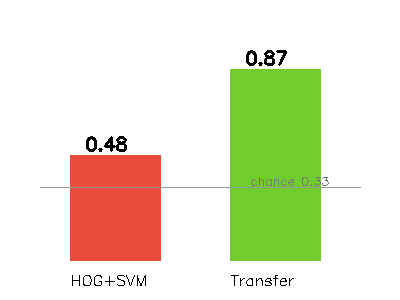
\includegraphics[width=0.95\linewidth]{../assets/accuracy_bars.png}
    \end{center}\end{column}
    \begin{column}{0.5\textwidth}
      \begin{itemize}
        \item \textbf{Same} 180 images, \textbf{same} SVM, \textbf{same} split.
        \item Only change: HOG $\rightarrow$ frozen ImageNet features.
        \item 0.48 $\rightarrow$ \textbf{0.87}. The features were the bottleneck all along.
      \end{itemize}
    \end{column}
  \end{columns}
\end{frame}

\begin{frame}{Confusion matrix after transfer}
  \begin{columns}[T]
    \begin{column}{0.5\textwidth}\begin{center}
      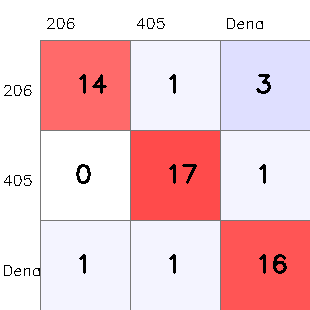
\includegraphics[width=0.95\linewidth]{../assets/confusion_transfer.png}
    \end{center}\end{column}
    \begin{column}{0.5\textwidth}
      \begin{itemize}
        \item The diagonal is now dominant — most cars classified correctly.
        \item Compare to Week 12's near-random confusion matrix.
        \item The pretrained net ``sees'' the fine differences HOG missed.
      \end{itemize}
    \end{column}
  \end{columns}
\end{frame}

\begin{frame}{A worked accuracy number}
  \begin{columns}[T]
    \begin{column}{0.52\textwidth}
      \begin{mathbox}[Reading the matrix]
        With 3 classes $\times$ 20 test images $=60$ tests, suppose the diagonal sums to 52:
        \[ \text{acc}=\frac{52}{60}=0.867 \approx 0.87 \]
      \end{mathbox}
      \begin{itemize}
        \item Per-class recall = (row diagonal) / (row total).
        \item One weak class can hide inside a good average — always read per-class.
      \end{itemize}
    \end{column}
    \begin{column}{0.48\textwidth}
      \begin{tabular}{@{}lccc@{}}
        \toprule
        & \multicolumn{3}{c}{predicted}\\
        true & A & B & C\\
        \midrule
        A & \textbf{18} & 1 & 1\\
        B & 2 & \textbf{17} & 1\\
        C & 1 & 2 & \textbf{17}\\
        \bottomrule
      \end{tabular}
      \\[3pt]
      {\scriptsize recall: A .90, B .85, C .85}
    \end{column}
  \end{columns}
\end{frame}

\begin{frame}{Why this works so well}
  \begin{itemize}
    \item ImageNet includes many vehicles — the net already learned car-relevant parts.
    \item Its mid-level features (grille shapes, light patterns) are exactly what separates models.
    \item We get the power of a huge net with only 60 images per class and seconds of training.
  \end{itemize}
  \begin{goodbox}
    Transfer learning is the single most useful deep-learning technique for real, small-data projects.
  \end{goodbox}
\end{frame}

% ==================================================================
\section{What transfers, and how far}
% ==================================================================

\begin{frame}{What each layer transfers}
  \begin{itemize}
    \item \term{Early layers}: edges, colours, textures — universal, transfer to \emph{any} task.
    \item \term{Middle layers}: parts and motifs — transfer well to related domains.
    \item \term{Late layers}: class-specific (``golden retriever'') — least transferable; often replaced.
  \end{itemize}
  \keyidea{The more your task differs from ImageNet, the more late layers you should retrain.}
\end{frame}

\begin{frame}{The domain gap}
  \begin{columns}[T]
    \begin{column}{0.56\textwidth}
      \begin{itemize}
        \item ImageNet is natural photos. Very different images (X-rays, thermal, tiny
              digits) transfer more weakly.
        \item Meters and cars are ordinary photos $\rightarrow$ small gap $\rightarrow$ transfer
              works great (our 0.87).
        \item Larger gap $\rightarrow$ fine-tune more layers, or find a model pretrained on
              closer data.
      \end{itemize}
    \end{column}
    \begin{column}{0.44\textwidth}
      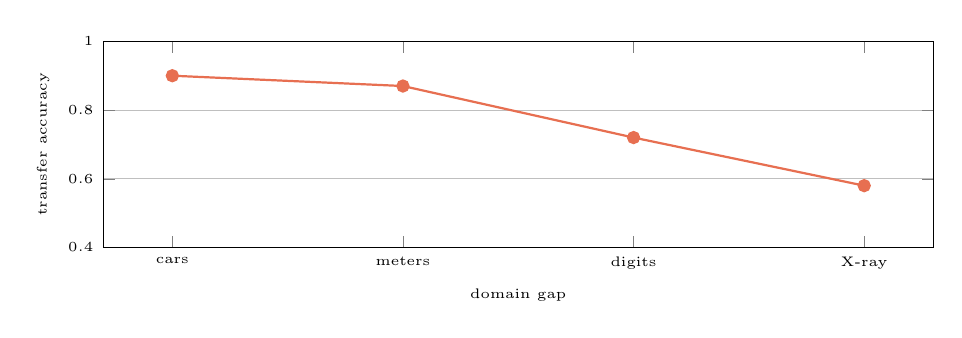
\begin{tikzpicture}[font=\tiny]
        \begin{axis}[width=\linewidth,height=4.2cm,
            xlabel={domain gap},ylabel={transfer accuracy},
            xtick={0,1,2,3},xticklabels={cars,meters,digits,X-ray},
            ymin=0.4,ymax=1,ymajorgrids]
          \addplot[courseAccent,thick,mark=*] coordinates
            {(0,0.90)(1,0.87)(2,0.72)(3,0.58)};
        \end{axis}
      \end{tikzpicture}
    \end{column}
  \end{columns}
  \begin{mathbox}
    Rule of thumb: small gap + small data $\rightarrow$ freeze \& extract; large gap + more data $\rightarrow$ fine-tune.
  \end{mathbox}
\end{frame}

% ==================================================================
\section{Squeezing more from small data}
% ==================================================================

\begin{frame}{Data augmentation for small data}
  \begin{itemize}
    \item Multiply your data for free: random flips, small rotations, brightness/contrast jitter, crops.
    \item Each variant teaches the same label under a new nuisance $\rightarrow$ more invariance, less overfitting.
    \item Especially valuable when combined with transfer learning on tiny datasets.
  \end{itemize}
  \begin{goodbox}
    Augmentation is the cheapest accuracy you will ever buy — always try it on small-data problems.
  \end{goodbox}
\end{frame}

\begin{frame}[fragile]{Augmentation, in practice (code)}
\begin{lstlisting}
aug = T.Compose([
    T.RandomHorizontalFlip(p=0.5),
    T.RandomRotation(8),                 # small: a car is still a car
    T.ColorJitter(brightness=0.2, contrast=0.2),
    T.RandomResizedCrop(224, scale=(0.8, 1.0)),
])
# make 5 augmented copies per training image, extract features on each
X = np.stack([features(aug(im)) for im in train_images for _ in range(5)])
\end{lstlisting}
  \begin{badbox}
    Only augment \emph{training} data, and only with label-preserving transforms — a vertical
    flip of a digit ``6'' is a lie.
  \end{badbox}
\end{frame}

\begin{frame}{Practical transfer-learning tips}
  \begin{itemize}
    \item Use the pretrained model's \emph{own} preprocessing (resize, normalize) — mismatch hurts a lot.
    \item Start with \term{feature extraction}; only fine-tune if you have enough data and need more.
    \item Freeze early layers (general), fine-tune late layers (task-specific) if you do fine-tune.
    \item Watch for overfitting — small data still bites; use augmentation and regularization.
  \end{itemize}
\end{frame}

% ==================================================================
\section{In-class exercise}
% ==================================================================

\begin{frame}{\faPen~In-class exercise (10 min)}
  \begin{infobox}[Reason it through]
  \end{infobox}
  \begin{enumerate}
    \item You have 40 images per class. From-scratch CNN or transfer learning? Why?
    \item Transfer learning lifted cars 0.48$\rightarrow$0.87 with the \emph{same} SVM. What changed, exactly?
    \item You standardize features on train+test together and your score jumps. Trust it? Why not?
    \item Your input is 128$\times$64 but the backbone expects 224$\times$224. What must you do first?
  \end{enumerate}
\end{frame}

\begin{frame}{\faPen~Debrief}
  \begin{itemize}
    \item (1) \term{Transfer learning} — 40 images is far too few to train a deep net from scratch without overfitting.
    \item (2) Only the \term{features}: hand-designed HOG $\rightarrow$ pretrained deep features. The classifier was identical.
    \item (3) \term{No} — fitting the scaler on test data leaks information; the gain is fake.
    \item (4) \term{Resize/normalize} with the backbone's own preprocessing before extracting.
  \end{itemize}
  \keyidea{Good ML engineering is mostly good \emph{features} and honest evaluation — not fancier models.}
\end{frame}

% ==================================================================
\section{Next session}
% ==================================================================

\begin{frame}{Next session: shipping DocScan}
  \begin{columns}[T]
    \begin{column}{0.6\textwidth}
      \begin{itemize}
        \item We can now \emph{read} the digits with transfer learning. Next: assemble the
              \term{whole DocScan pipeline} end to end.
        \item Every week of the course was one stage — we bolt them together.
        \item Then: engineering for the real world (confidence gates, fallbacks) and the
              \term{capstone deliverable}.
      \end{itemize}
    \end{column}
    \begin{column}{0.4\textwidth}
      \begin{alertblock}{Come ready}
        Re-skim your Week 11 homography and Week 9 contour code — you'll wire them in.
      \end{alertblock}
    \end{column}
  \end{columns}
\end{frame}

\begin{frame}[standout]
  Better features, not a bigger model.\\[4pt]
  \normalsize A frozen giant did the seeing; a tiny SVM did the deciding — 0.48 to 0.87.
\end{frame}

\end{document}
